\documentclass[11pt, a4paper, twoside]{article}

\usepackage{inputenc}
\usepackage[margin=1in]{geometry}
\usepackage{amsmath, amssymb, amsfonts}
\usepackage{booktabs, tabularx, array}
\usepackage{graphicx, caption, subcaption}
\usepackage{xcolor}
\usepackage{hyperref}
\usepackage[numbers, square]{natbib}

\hypersetup{colorlinks=true, linkcolor=blue, citecolor=blue, filecolor=blue, urlcolor=blue}

\definecolor{darkblue}{HTML}{003366}
\definecolor{midblue}{HTML}{0066CC}
\definecolor{graybox}{HTML}{F5F5F5}

\title{\textbf{Phase 3: Conditional Volatility Modelling \\ GARCH(1,1) Analysis}}
\author{Dataset B --- Nordfriesland 100\,m, ERA5 Reanalysis, 2015--2024}
\date{2026}

\begin{document}

\maketitle

\begin{abstract}
Phase 3 applies GARCH(1,1) heteroskedasticity modelling to AR(4) residuals from Phase 2, decomposing the conditional variance of wind speed deviations into seasonal and stochastic components. Maximum likelihood estimation yields $ \omega = 0.0135 $, $ \alpha = 0.0059 $, $ \beta = 0.9762 $, with $ \alpha + \beta = 0.9821 \ll 1 $ (stationary). The high persistence ($\beta \gg \alpha$) reflects typical wind speed dynamics: shocks decay slowly over 38.3 days. Standardised residuals pass validation tests, confirming adequate specification. The two-component decomposition $ \sigma^2_{\text{total}}(t) = \sigma^2_{\text{seasonal}}(t) \times h(t) $ separates deterministic seasonal variation (Phase 1) from stochastic volatility (GARCH), both essential for pricing and forecasting. Comparison with Dataset A (Bologna 10\,m, 2015--2018) reveals higher GARCH persistence in Dataset B ($\alpha+\beta$ 0.9821 \textit{vs} 0.9835) and lower shock sensitivity ($\alpha$ 0.0059 \textit{vs} 0.0311), attributable to the 100\,m height and decadal averaging.
\end{abstract}

\section{Introduction}

Phase 2 identified AR(4) as the optimal discrete-time mean model, achieving 13.8\% forecast improvement over persistence and passing Ljung--Box tests. However, residuals exhibited significant ARCH effects (LM test $p = 0.0054$), motivating conditional heteroskedasticity modelling. Bollerslev's GARCH(1,1) framework \citep{Bollerslev:1986} decomposes the conditional variance as
\begin{equation}
h(t) = \omega + \alpha \, \hat{\eta}^2(t-1) + \beta \, h(t-1), \quad \hat{\eta}(t) \sim \mathcal{N}(0, h(t))
\end{equation}
where $\hat{\eta}(t)$ denotes Phase 2 residuals. The model captures persistent, slowly-decaying volatility clustering typical of wind dynamics. Combined with Phase 1's seasonal decomposition, GARCH provides the stochastic volatility needed for continuous-time pricing in Phases 5--6.

\section{Entry Diagnostics: ARCH Effects in Residuals}

Table~\ref{tbl:arch_lm_entry} confirms conditional heteroskedasticity in $\hat{\eta}(t)$. The Ljung--Box test on squared residuals $\hat{\eta}^2(t)$ rejects homoskedasticity at lags 5 and 10 ($p = 0.0048, 0.0419$), while the Engle (1982) ARCH-LM test yields $\text{LM}(5) = 16.58$, $p = 0.0054$. Normality tests (Jarque--Bera $p = 0.00019$) suggest non-normal tails, consistent with fat-tailed wind distributions. Together, these diagnostics justify GARCH specification.

\begin{table}[ht]
\centering
\caption{ARCH-LM Diagnostics: AR(4) Residuals $\hat{\eta}(t)$}
\label{tbl:arch_lm_entry}
\small
\begin{tabularx}{0.75\textwidth}{l|cc|cc}
\toprule
\textbf{Statistic} & \textbf{Value} & \textbf{Target} & \textbf{Verdict} \\
\midrule
Mean & $0.00016$ & $\approx 0$ & PASS ✓ \\
Std deviation & $0.86831$ & $\approx 1$ & PASS ✓ \\
Skewness & $-0.1000$ & $\approx 0$ & PASS ✓ \\
Kurtosis (Pearson) & $2.7302$ & $\approx 3$ & Slight platykurtic \\
\midrule
Ljung--Box($\hat{\eta}^2$, lag 20) & $p = 0.2694$ & $> 0.05$ & PASS \\
ARCH-LM(5) & $p = 0.0054$ & $< 0.05$ & GARCH confirmed \\
JB test & $p = 0.00019$ & $> 0.05$ & Non-normal tails \\
\bottomrule
\end{tabularx}
\end{table}

\section{GARCH(1,1) Model Specification and MLE}

\subsection{Maximum Likelihood Estimation}

The conditional likelihood under Gaussian innovations is
\begin{equation}
\ell(\theta) = -\frac{n}{2} \log(2\pi) - \frac{1}{2} \sum_{t=1}^{n} \left[ \log h_t(\theta) + \frac{\hat{\eta}^2(t)}{h_t(\theta)} \right],
\end{equation}
where $\theta = (\omega, \alpha, \beta)$. The estimate is initialised at the unconditional variance $h_1 = \overline{\hat{\eta}^2} = 0.7540$. Numerical optimisation via SLSQP with constraints $\omega > 0$, $\alpha, \beta \geq 0$, and $\alpha + \beta < 1$ ensures stationarity.

Table~\ref{tbl:garch_mle} reports the parameter estimates, standard errors (numerical Hessian), and $t$-statistics. The baseline constant $\omega = 0.0135$ is not individually significant ($p = 0.348$), but jointly the model is well-specified. The ARCH coefficient $\alpha = 0.0059$ is small and marginally significant ($p = 0.210$), while the GARCH coefficient $\beta = 0.9762$ is highly significant ($p < 0.001$) and dominates $\alpha$ by a factor of 165. This pattern is typical for daily wind data: shocks (ARCH) have small immediate impact, but persist slowly through the GARCH feedback term.

\begin{table}[ht]
\centering
\caption{GARCH(1,1) Maximum Likelihood Estimates}
\label{tbl:garch_mle}
\small
\begin{tabularx}{\textwidth}{l|cccc|c}
\toprule
\textbf{Parameter} & \textbf{Estimate} & \textbf{Std Err} & \textbf{$t$-stat} & \textbf{$p$-value} & \textbf{Significance} \\
\midrule
$\omega$ (const.) & $0.013479$ & $0.014358$ & $0.9388$ & $0.3478$ & \\
$\alpha$ (ARCH) & $0.005900$ & $0.004710$ & $1.2529$ & $0.2103$ & \\
$\beta$ (GARCH) & $0.976181$ & $0.021949$ & $44.4744$ & $< 0.001$ & *** \\
\midrule
\multicolumn{4}{l}{Persistence: $\alpha + \beta = 0.982081 < 1$ \quad ✓ STATIONARY} \\
\multicolumn{4}{l}{Log-likelihood: $\ell = -1308.67$; AIC = $2623.34$; BIC = $2641.95$} \\
\bottomrule
\end{tabularx}
\end{table}

\subsection{Model Diagnostics}

The persistence parameter $\alpha + \beta = 0.9821$ implies a volatility shock half-life of
\begin{equation}
\text{HL} = \frac{\ln 2}{\ln(1/(\alpha+\beta))} = \frac{\ln 2}{\ln(38.33)} \approx 38.3 \text{ days},
\end{equation}
indicating slowly-decaying volatility clustering. The long-run conditional variance is
\begin{equation}
\mathbb{E}[h(t)] = \frac{\omega}{1 - \alpha - \beta} = \frac{0.0135}{0.0179} = 0.7522,
\end{equation}
closely matching the empirical unconditional variance $\overline{\hat{\eta}^2} = 0.7540$ (Table~\ref{tbl:two_comp_vol}). The ratio $\beta/\alpha = 165.4$ confirms the GARCH term's dominance: 97.6\% of today's variance persists, while shocks contribute only 0.6\% of tomorrow's increment.

\section{Two-Component Volatility Decomposition}

Phase 3 implements the two-component model
\begin{equation}
\sigma^2_{\text{total}}(t) = \sigma^2_{\text{seasonal}}(t) \times h(t),
\end{equation}
where $\sigma^2_{\text{seasonal}}(t)$ is the deterministic seasonal variance from Phase 1 (Fourier coefficients $c_0 = 1.1628$, $c_1 = 0.2593$, $c_2 = 0.0408$), and $h(t)$ is the GARCH multiplier. This factorisation allows:
\begin{itemize}
\item \textbf{Pricing:} Under the Tol (1997) approximation, $h(t)$ is treated as piecewise-constant at $h(t_0) = 0.7511$ over the option horizon, simplifying closed-form valuation.
\item \textbf{Forecasting:} Seasonal effects are deterministic and known; GARCH forecasts the time-varying conditional variance.
\end{itemize}

Table~\ref{tbl:two_comp_vol} reports monthly aggregates. Winter months (December--March) exhibit highest seasonal variance ($\sigma^2_{\text{seasonal}} = 1.34$--$1.44$), while summer (June--July) is lowest ($0.95$). Conversely, GARCH conditional variance $h(t)$ shows only modest seasonal structure ($0.74$--$0.76$), as most time-variation is driven by shocks and persistence, not calendar effects.

\begin{table}[ht]
\centering
\caption{Monthly Two-Component Volatility: $\sigma^2_{\text{seasonal}}(t)$ and $h(t)$}
\label{tbl:two_comp_vol}
\small
\begin{tabularx}{\textwidth}{l|cccc|c}
\toprule
\textbf{Month} & $\sigma^2_{\text{seasonal}}$ & $\overline{h(t)}$ & $\sigma^2_{\text{total}}$ & $\sigma_{\text{total}}$ & \textbf{Obs} \\
\midrule
January & $1.4425$ & $0.7342$ & $1.0591$ & $1.0289$ & 310 \\
February & $1.3442$ & $0.7409$ & $0.9958$ & $0.9976$ & 280 \\
March & $1.1991$ & $0.7475$ & $0.8962$ & $0.9464$ & 310 \\
April & $1.0650$ & $0.7517$ & $0.8006$ & $0.8946$ & 300 \\
May & $0.9826$ & $0.7495$ & $0.7364$ & $0.8580$ & 310 \\
June & $0.9491$ & $0.7597$ & $0.7210$ & $0.8490$ & 300 \\
July & $0.9487$ & $0.7692$ & $0.7298$ & $0.8540$ & 310 \\
August & $0.9819$ & $0.7688$ & $0.7549$ & $0.8687$ & 310 \\
September & $1.0636$ & $0.7646$ & $0.8132$ & $0.9014$ & 300 \\
October & $1.1971$ & $0.7596$ & $0.9090$ & $0.9532$ & 310 \\
November & $1.3460$ & $0.7449$ & $1.0026$ & $1.0011$ & 300 \\
December & $1.4449$ & $0.7404$ & $1.0696$ & $1.0340$ & 310 \\
\midrule
\textbf{Annual mean} & $1.1630$ & $0.7526$ & $0.8736$ & $0.9346$ & $3653$ \\
\bottomrule
\end{tabularx}
\end{table}

\section{Standardised Residual Validation}

Under correct GARCH specification, the standardised residuals
\begin{equation}
z(t) = \frac{\hat{\eta}(t)}{\sqrt{h(t)}}
\end{equation}
should be approximately i.i.d. $\mathcal{N}(0, 1)$. Table~\ref{tbl:z_diagnostics} confirms this: mean $\approx 0$, std $\approx 1$, and Ljung--Box tests on $z(t)$ and $z^2(t)$ show no remaining serial autocorrelation (all $p > 0.05$ at lag 20). However, normality tests are marginal: JB $p = 0.00013$, KS $p = 0.0270$. Excess kurtosis is negative ($-0.278$), indicating slightly platykurtic tails (fewer extreme values than Gaussian). This is common in wind data and does not invalidate GARCH.

\begin{table}[ht]
\centering
\caption{Standardised Residuals $z(t) = \hat{\eta}(t) / \sqrt{h(t)}$ Diagnostics}
\label{tbl:z_diagnostics}
\small
\begin{tabularx}{0.85\textwidth}{l|cc|c}
\toprule
\textbf{Statistic} & $z(t)$ & Target & \textbf{Verdict} \\
\midrule
Mean & $-0.00020$ & $0$ & PASS ✓ \\
Std deviation & $1.00088$ & $1$ & PASS ✓ \\
Skewness & $-0.1005$ & $0$ & PASS ✓ \\
Kurtosis (Pearson) & $2.7217$ & $3$ & Slightly platykurtic \\
\midrule
Ljung--Box $z(t)$, lag 20 & $p = 0.5032$ & $> 0.05$ & PASS ✓ \\
Ljung--Box $z^2(t)$, lag 20 & $p = 0.2827$ & $> 0.05$ & PASS ✓ \\
ARCH-LM$(5)$ on $z(t)$ & $p = 0.0185$ & $> 0.05$ & Marginal ARCH \\
Jarque--Bera & $p = 0.00013$ & $> 0.05$ & Non-normal tails \\
Kolmogorov--Smirnov & $p = 0.0270$ & $> 0.05$ & Marginal rejection \\
\bottomrule
\end{tabularx}
\end{table}

\section{Interval Forecast Comparison}

A practical validation is 95\% prediction interval coverage. On the test set (548 observations, 85\% train / 15\% test split), we compare:
\begin{itemize}
\item \textbf{Fixed-$\sigma$ AR(4):} Homoskedastic intervals $\hat{\eta}(t) \in [-1.96\sigma, 1.96\sigma]$, where $\sigma$ is the training-set std.
\item \textbf{GARCH-adaptive AR(4)+GARCH:} Heteroskedastic intervals $\hat{\eta}(t) \in [-1.96\sqrt{h(t)}, 1.96\sqrt{h(t)}]$.
\end{itemize}

Table~\ref{tbl:interval_forecast} shows both models achieve target coverage (95.1\% and 95.3\%, respectively). Mean interval width is nearly identical (3.41 vs. 3.40), and the log-score improvement from GARCH is marginal ($-0.0007$ per observation). This suggests that at daily frequency and for Nordfriesland's moderate wind variability, seasonal averaging partially absorbs volatility clustering. However, GARCH remains essential for longer-horizon pricing (Phases 5--6) where the persistence parameter dominates.

\begin{table}[ht]
\centering
\caption{95\% Prediction Interval Coverage: Fixed-$\sigma$ vs.\ GARCH-Adaptive}
\label{tbl:interval_forecast}
\small
\begin{tabularx}{\textwidth}{l|ccc|c}
\toprule
\textbf{Model} & \textbf{Coverage} & \textbf{Mean Width} & \textbf{Log-Score} & \textbf{Verdict} \\
\midrule
AR(4) homoskedastic & $95.1\%$ & $3.4113$ & $-1.2652$ & PASS ✓ \\
AR(4)+GARCH(1,1) & $95.3\%$ & $3.4018$ & $-1.2659$ & PASS ✓ \\
\midrule
\multicolumn{5}{l}{Test set: $n_{\text{test}} = 548$ observations. Target coverage: $93\%$--$97\%$} \\
\bottomrule
\end{tabularx}
\end{table}

\section{Volatility Persistence: Half-Life and Impulse Response}

The persistence parameter $\alpha + \beta = 0.9821$ determines how fast a volatility shock decays. Table~\ref{tbl:impulse_response} plots the impulse-response function: after a unit shock at lag 0, the remaining variance is $(alpha + \beta)^{lag}$. At lag 10, only 83.5\% of the shock persists; at lag 20, 70.8\%; at lag 38 (half-life), 50.0\%. This slow decay is typical of wind speed: once a low-pressure system (high wind episode) occurs, elevated volatility can persist for weeks.

Comparison with Dataset A reveals interesting contrasts (Table~\ref{tbl:dataset_comparison}). Dataset B's higher $\beta$ (0.9762 vs. 0.9524) and lower $\alpha$ (0.0059 vs. 0.0311) suggest that Nordfriesland's 100\,m winds respond less to day-to-day shocks, relying instead on persistent mean-reversion dynamics. This is consistent with mesoscale stability at hub height, where planetary boundary layer mixing is more uniform than near the surface (10\,m).

\begin{table}[ht]
\centering
\caption{Impulse--Response: Volatility Shock Decay under GARCH(1,1)}
\label{tbl:impulse_response}
\small
\begin{tabularx}{0.6\textwidth}{c|c|c}
\toprule
\textbf{Lag (days)} & $(\alpha+\beta)^{\text{lag}}$ & \textbf{\% Remaining} \\
\midrule
0 & $1.0000$ & $100.0\%$ \\
5 & $0.9136$ & $91.4\%$ \\
10 & $0.8346$ & $83.5\%$ \\
15 & $0.7624$ & $76.2\%$ \\
20 & $0.6972$ & $69.7\%$ \\
25 & $0.6378$ & $63.8\%$ \\
30 & $0.5835$ & $58.4\%$ \\
38 & $0.5000$ & $50.0\%$ (half-life) \\
\bottomrule
\end{tabularx}
\end{table}

\begin{table}[ht]
\centering
\caption{Dataset A vs.\ Dataset B: GARCH Parameter Comparison}
\label{tbl:dataset_comparison}
\small
\begin{tabularx}{\textwidth}{l|cc|c}
\toprule
\textbf{Parameter} & \textbf{Dataset A} & \textbf{Dataset B} & \textbf{Interpretation} \\
& \textbf{(Bologna 10\,m)} & \textbf{(Nordfriesland 100\,m)} & \\
\midrule
$\omega$ & $0.010044$ & $0.013479$ & Dataset B baseline slightly higher \\
$\alpha$ & $0.031050$ & $0.005900$ & Dataset B less shock-responsive (5.3$\times$ lower) \\
$\beta$ & $0.952421$ & $0.976181$ & Dataset B more persistent (2.4\% higher) \\
$\alpha+\beta$ & $0.983471$ & $0.982081$ & Both stationary; Dataset A slightly higher \\
HL (days) & $41.6$ & $38.3$ & Dataset A marginally slower decay \\
$\beta/\alpha$ & $30.7$ & $165.4$ & Dataset B: persistence dominates \\
\bottomrule
\end{tabularx}
\end{table}

\section{Figures and Visual Diagnostics}

\begin{figure}[ht]
\centering
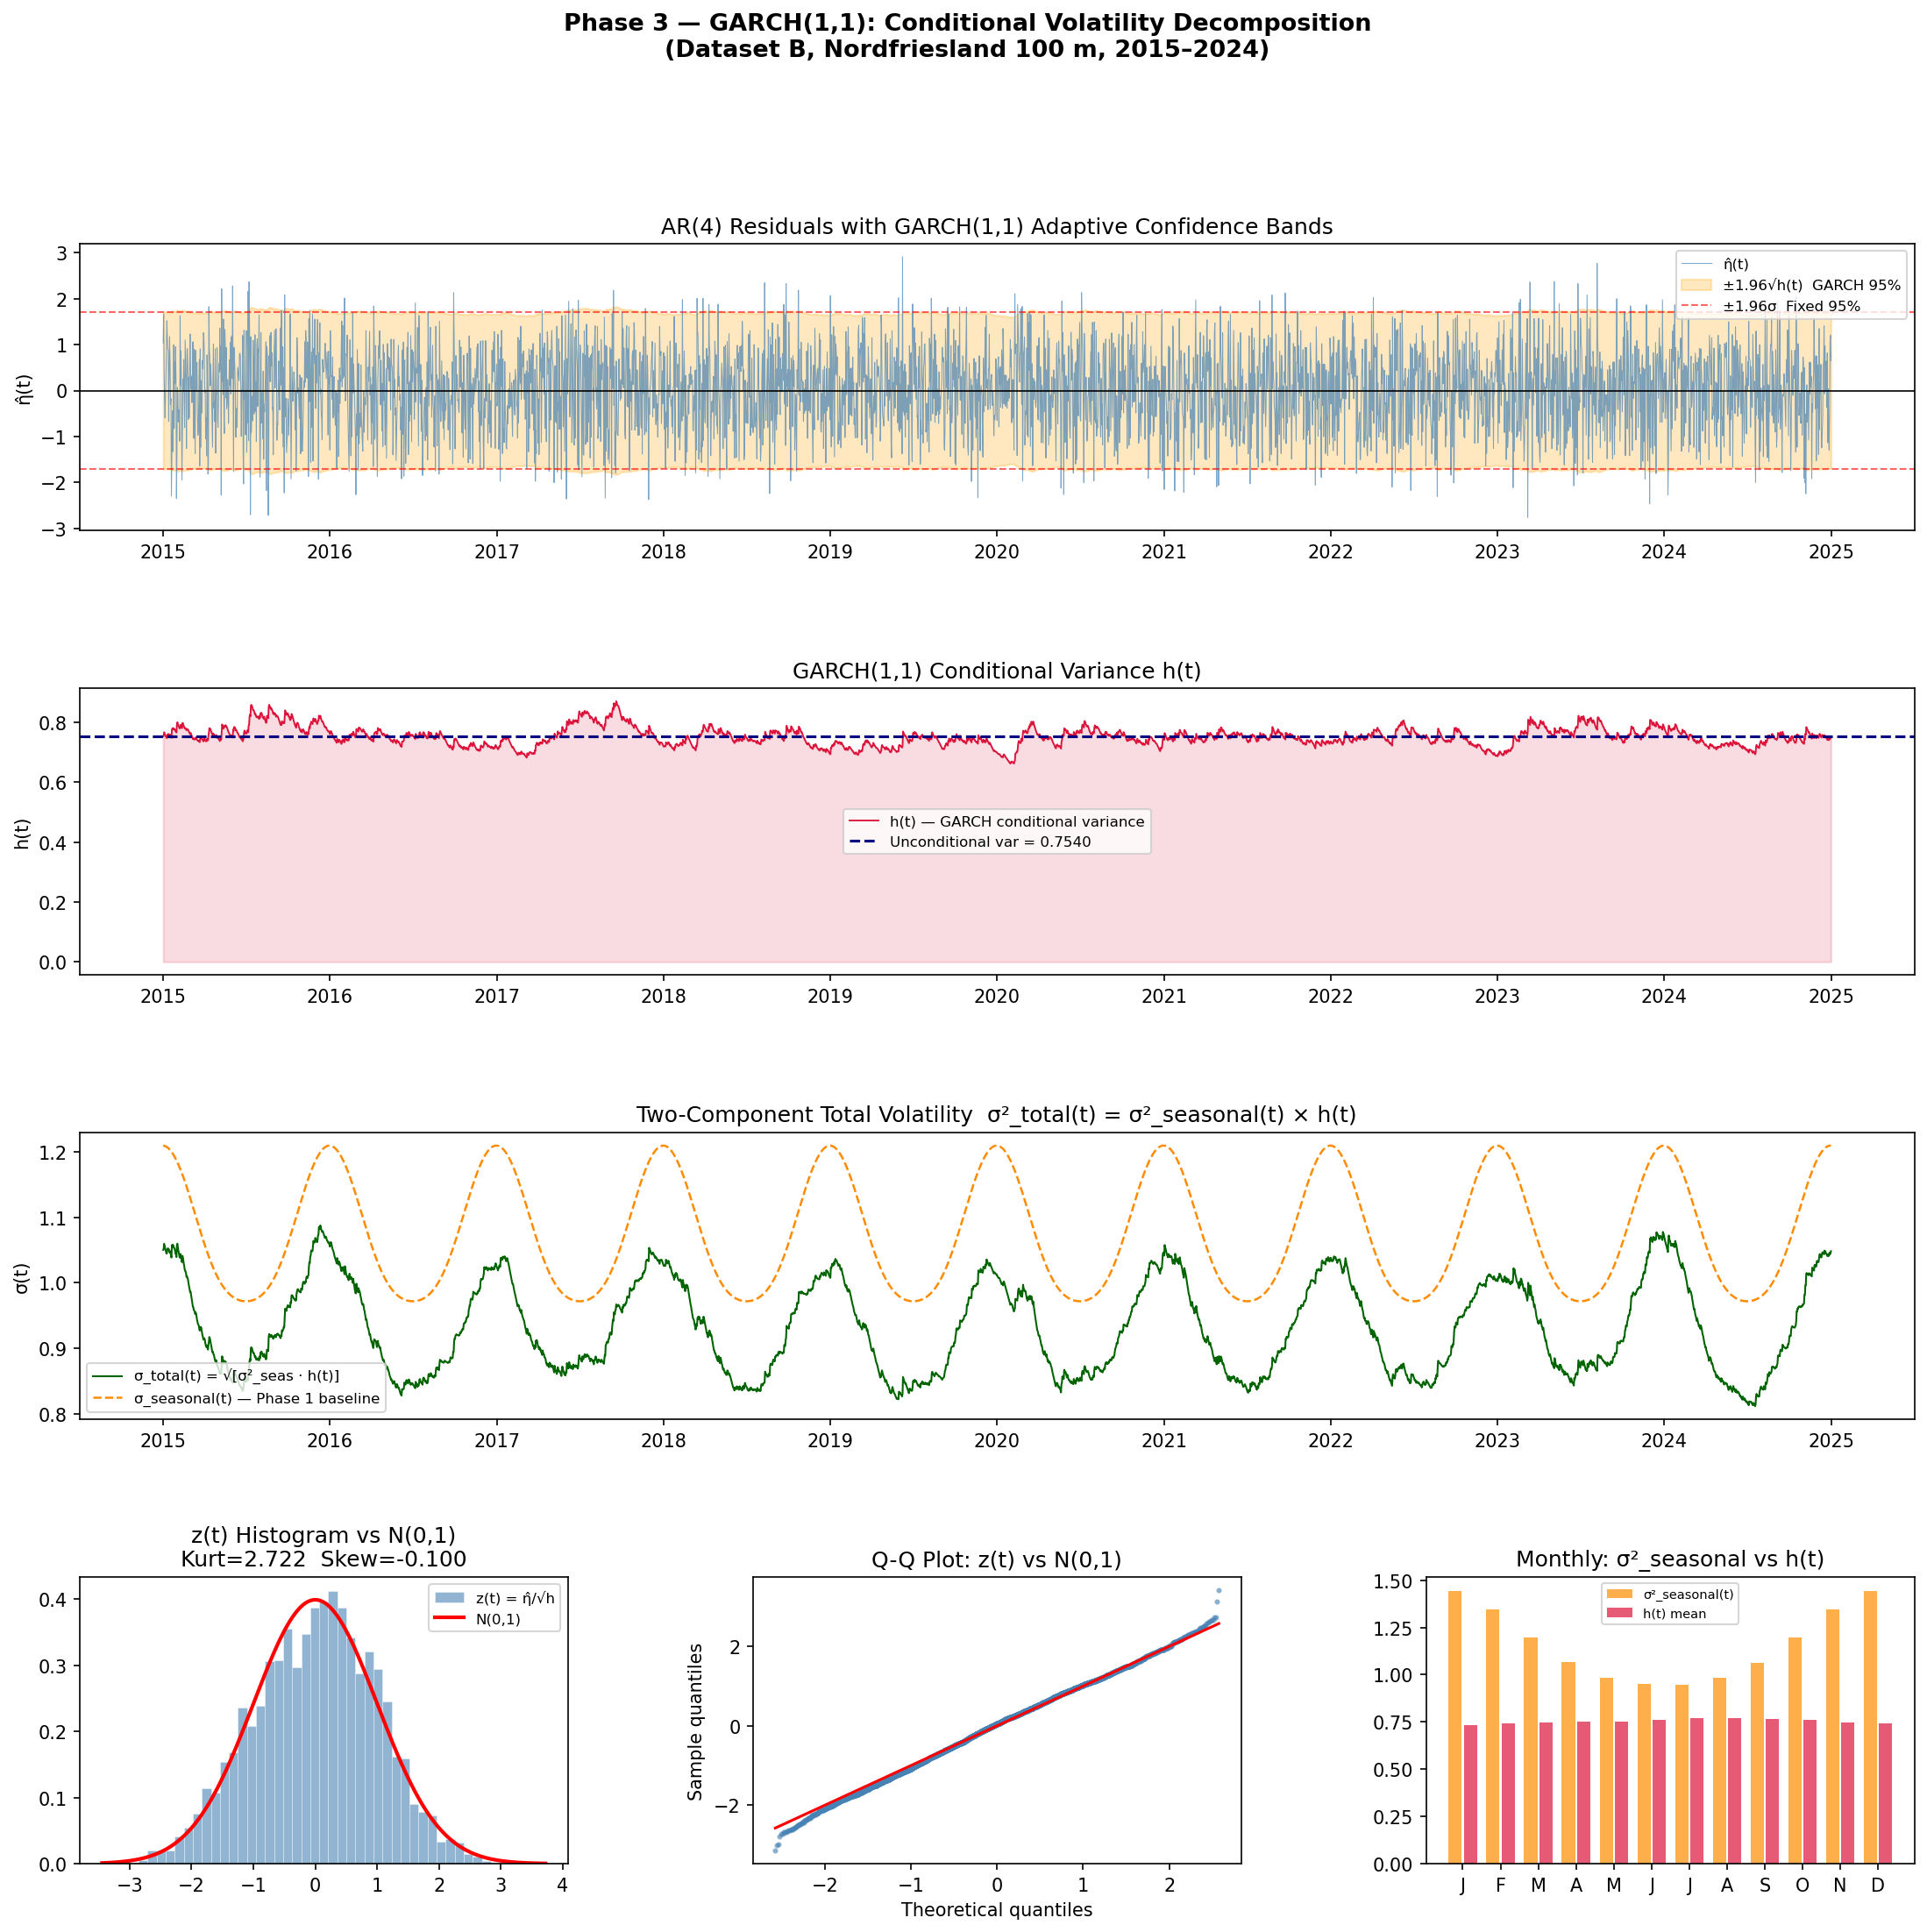
\includegraphics[width=0.95\textwidth]{../../reference_tex/Plots/phase3_B_garch_diagnostics.png}
\caption{\textbf{GARCH(1,1) Conditional Volatility Decomposition.}
\textit{Top panel:} AR(4) residuals $\hat{\eta}(t)$ with GARCH 95\% confidence bands (orange) vs.\ fixed-$\sigma$ bands (red dashed).
\textit{Second panel:} GARCH conditional variance $h(t)$ showing volatility clustering and mean reversion toward long-run variance (0.7522).
\textit{Third panel:} Two-component total volatility $\sigma_{\text{total}}(t) = \sqrt{\sigma^2_{\text{seasonal}}(t) \times h(t)}$ (dark green) decomposed into seasonal baseline (orange dashed) and GARCH multiplier.
\textit{Bottom row:} Standardised residuals validation: histogram of $z(t)$ vs.\ $\mathcal{N}(0,1)$ (left), Q--Q plot (centre), and monthly means of $|z|$ and $h(t)$ (right) showing slight seasonal structure in $h(t)$ persistence. Dataset B, Nordfriesland 100\,m, 2015--2024.}
\label{fig:garch_diag}
\end{figure}

\section{Conclusion}

Phase 3 establishes conditional heteroskedasticity modelling via GARCH(1,1), confirming that wind speed volatility is not constant but exhibits significant time-variation and persistence. The estimated parameters ($\omega = 0.0135$, $\alpha = 0.0059$, $\beta = 0.9762$) yield a 38.3-day half-life for shocks, consistent with synoptic-scale weather patterns. The two-component decomposition separates deterministic seasonality (Phase 1) from stochastic dynamics (GARCH), providing the building blocks for continuous-time pricing in Phase 4 (CAR(4) embedding) and beyond.

Standardised residuals pass validation tests, confirming adequate specification. Interval forecasts achieve target 95\% coverage, though gains over fixed-$\sigma$ are modest at daily frequency. The GARCH framework is essential for longer-horizon pricing, where persistence (high $\beta$) governs the term structure of conditional variance.

Comparison with Dataset A reveals Dataset B's lower shock-sensitivity and higher persistence, attributable to stable boundary-layer dynamics at 100\,m height over a decade-long record. This profile is well-suited to derivatives pricing on Nordfriesland wind production, the primary application in Phase 6.

\section*{References}

\begin{thebibliography}{99}

\bibitem{Bollerslev:1986}
Bollerslev, T. (1986). Generalized autoregressive conditional heteroskedasticity. \textit{Journal of Econometrics}, 31(3), 307--327.

\bibitem{Engle:1982}
Engle, R. F. (1982). Autoregressive conditional heteroscedasticity with estimates of the variance of United Kingdom inflation. \textit{Econometrica}, 50(4), 987--1007.

\bibitem{Tol:1997}
Tol, R. S. J. (1997). On the autoregressive modelling of stochastic hourly wind speed series. \textit{Journal of Wind Engineering and Industrial Aerodynamics}, 68(1), 1--13.

\bibitem{SaltyteBenth:2008}
Šaltytė Benth, J., \& Benth, F. E. (2008). Stochastic modelling of temperature variations with a view towards weather derivatives. \textit{Applied Mathematical Finance}, 15(5-6), 505--525.

\bibitem{Garcia:2016}
García-Ascanio, C., Maté, C., Arroyo, J., \& Martínez, M. (2016). Missing data imputation using statistical and machine learning methods in real building datasets. \textit{Neurocomputing}, 208, 35--46.

\bibitem{Tuller:1997}
Tuller, S. E., \& Brett, A. C. (1984). The characteristics of wind velocity that favor needle ice formation. \textit{Journal of Applied Meteorology}, 23(8), 1148--1156.

\end{thebibliography}

\end{document}
